 \documentclass[a4paper,10pt]{article}
\input{/Users/WannaGetHigh/workspace/latex/macros.tex}

\title{TP RdF, semaine 12: cha�nes, langages et grammaires}
\author{Fran�ois \bsc{Lepan}}

\begin{document}
\maketitle

\section{Distance de cha�nes}
\subsection{� la main}


\begin{tabular}{|c|c|c|c|c|c|c|c|c|}
\hline
& & e & x & c & u & s & e & d \\
 \hline
  & 0 & 1 & 2 & 3 & 4 & 5 & 6 & 7 \\
\hline
 e &1 & 0 & 1 & 2 & 3 & 4 & 5 & 6 \\
 \hline
 x & 2 & 1 & 0 & 1 & 2 & 3 & 4 & 5 \\
\hline
 h & 3 & 2 & 1 & 1 & 2 & 3 & 4 & 5 \\
\hline
 a & 4 & 3 & 2 & 2 & 2 & 3 & 4 & 5 \\
\hline
 u & 5 & 4 & 3 & 3 & 2 & 3 & 4 & 5 \\
\hline
 s & 6 & 5 & 4 & 4 & 3 & 2 & 3 & 4 \\
\hline
 t & 7 & 6 & 5 & 5 & 4 & 3 & 3 & 4 \\
\hline
 e & 8 & 7 & 6 & 6 & 5 & 4 & 3 & 4 \\
\hline
 d & 9 & 8 & 7 & 7 & 6 & 5 & 4 & 3 \\
\hline
\end{tabular}

\subsection{Sur machine}

\begin{paragraph}{Pour 'abacc'}
\begin{verbatimtab}
?- levenshtein('abacc','aabbc',D).
D = 3.
?- levenshtein('abacc','ababcc',D).       Distance moyenne = 2.
D = 1.
?- levenshtein('abacc','babbcc',D).
D = 2.

?- levenshtein('abacc','bccba',D).
D = 4.
?- levenshtein('abacc','bbbca',D).         Distance moyenne = 4
D = 3.
?- levenshtein('abacc','cbbaaaa',D).
D = 5.

?- levenshtein('abacc','caaaa',D).
D = 4.
?- levenshtein('abacc','cbcaab',D).       Distance moyenne = 3.6
D = 4.
?- levenshtein('abacc','baaca',D).
D = 3.
\end{verbatimtab}

Donc 'abacc' appartient � la classe 1.
\end{paragraph}

\begin{paragraph}{Pour 'ccab'}
\begin{verbatimtab}
?- levenshtein('ccab','aabbc',D).
D = 4.
?- levenshtein('ccab','ababcc',D).        Distance moyenne = 4.33
D = 4.
?- levenshtein('ccab','babbcc',D).
D = 5.

?- levenshtein('ccab','bccba',D).
D = 3.
?- levenshtein('ccab','bbbca',D).          Distance moyenne = 4
D = 4.
?- levenshtein('ccab','cbbaaaa',D).
D = 5.

?- levenshtein('ccab','caaaa',D).
D = 3.
?- levenshtein('ccab','cbcaab',D).        Distance moyenne = 3
D = 2.
?- levenshtein('ccab','baaca',D).
D = 4.
\end{verbatimtab}

Donc 'ccab' appartient � la classe 3.
\end{paragraph}

\begin{paragraph}{Pour 'ccbba'}
\begin{verbatimtab}

?- levenshtein('ccbba','aabbc',D).
D = 3.
?- levenshtein('ccbba','ababcc',D).       Distance moyenne = 4
D = 5.
?- levenshtein('ccbba','babbcc',D).
D = 4.

?- levenshtein('ccbba','bccba',D).
D = 2.
?- levenshtein('ccbba','bbbca',D).      Distance moyenne = 3
D = 3.
?- levenshtein('ccbba','cbbaaaa',D).
D = 4.

?- levenshtein('ccbba','caaaa',D).
D = 3.
?- levenshtein('ccbba','cbcaab',D).       Distance moyenne = 3.66
D = 4.
?- levenshtein('ccbba','baaca',D).
D = 4.
\end{verbatimtab}

Donc 'ccbba' appartient � la classe 2
\end{paragraph}

\begin{paragraph}{Pour 'bbaaac'}
\begin{verbatimtab}
?- levenshtein('bbaaac','aabbc',D).
D = 4.
?- levenshtein('bbaaac','ababcc',D).      Distance moyenne = 3.66
D = 3.
?- levenshtein('bbaaac','babbcc',D).
D = 4.

?- levenshtein('bbaaac','bccba',D).
D = 4.
?- levenshtein('bbaaac','bbbca',D).        Distance moyenne = 3
D = 3.
?- levenshtein('bbaaac','cbbaaaa',D).
D = 2.

?- levenshtein('bbaaac','caaaa',D).
D = 3.
?- levenshtein('bbaaac','cbcaab',D).       Distance moyenne = 3
D = 3.
?- levenshtein('bbaaac','baaca',D).
D = 3.
\end{verbatimtab}

Donc 'bbaaac' peut �tre de classe 2 ou de classe 3
\end{paragraph}


\section{Arbre de d�rivation pour une grammaire}
\subsection{A la main : la grammaire G}
\begin{verbatimtab}
  - Alphabet A = {a,b,c}
  - Axiome = S
  - Non-terminaux = {A,B}
  - R�gles de production P =
	S --> cAb
	A --> aBa
	B --> aBa
	B --> cb
\end{verbatimtab}
\subsubsection{De quel type est cette grammaire?}

C'est une grammaire alg�brique car elle est de la forme $R_i:T\rightarrow x$ o� x est terminal ou non

\subsection{Montrez que cette grammaire g�n�re le langage L(G) = \{$c a^n cb a^n b$ | $n \geq 1$\}}

On peut voir sur la Fig.~\ref{grammar_abc} que � chaque fois on rajoute autant de a de chaque cot� du cb centrale (cas d'arr�t). 

\begin{figure}[ht]
\begin{center}
	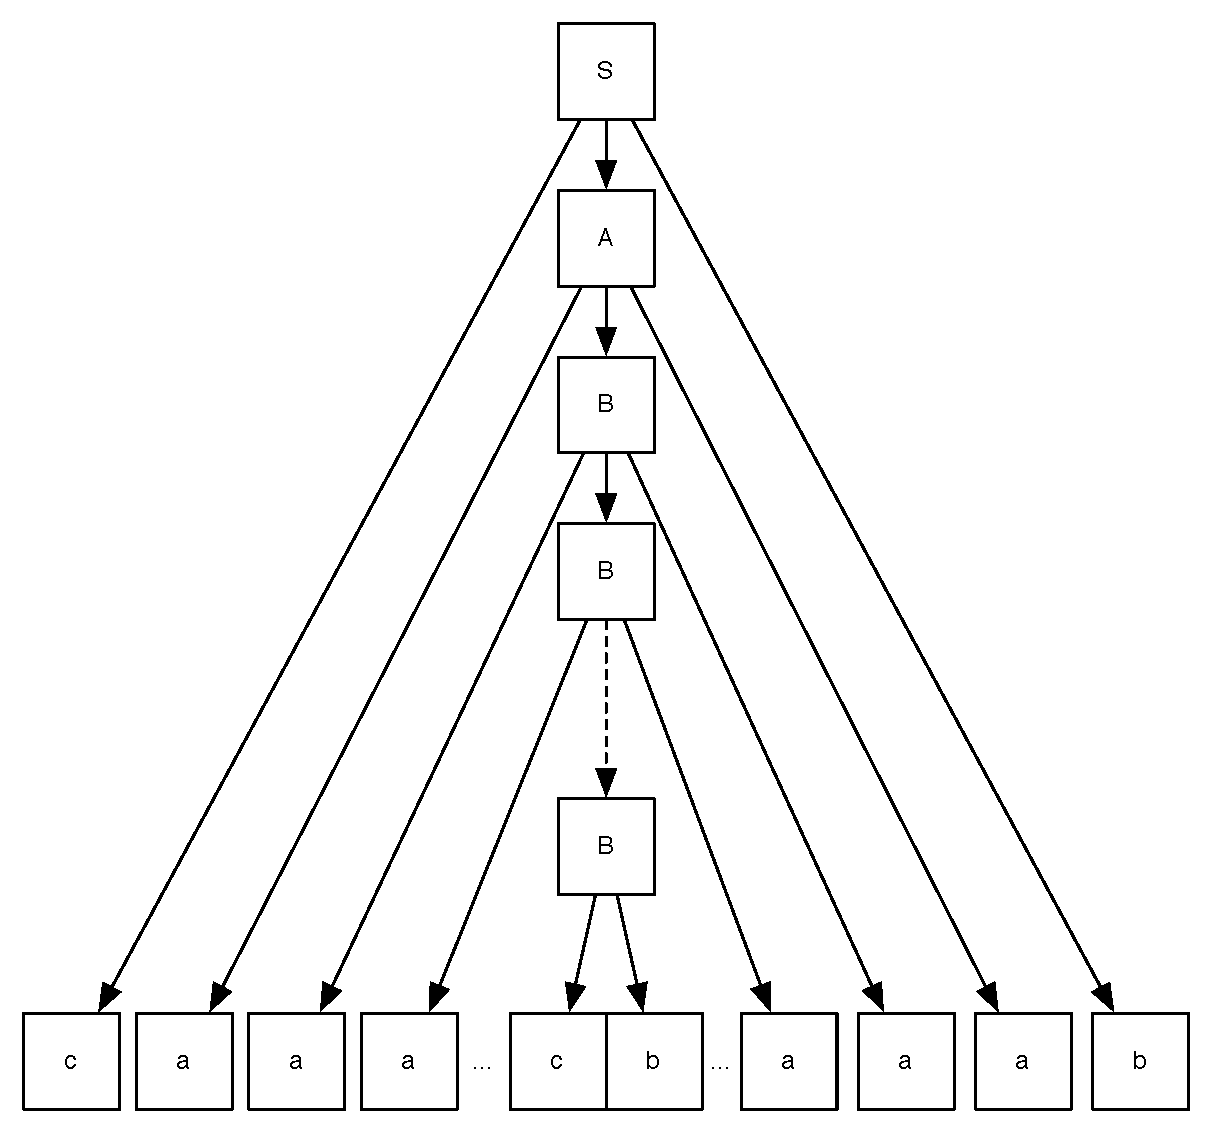
\includegraphics[width=15cm]{figures/grammar_abc}
\end{center}
	\caption{Arbre de d�rivation de la grammaire G}
	\label{grammar_abc}
\end{figure}\subsection{Arbres de d�rivation}



\end{document}